\documentclass[utf8]{beamer}
\mode<presentation>
\usepackage[spanish]{babel}
\usepackage{multicol}
\useoutertheme{infolines} 
\usepackage{graphicx}
\usetheme{boxes} % other themes: AnnArbor, Antibes, Bergen, Berkeley, Berlin, Boadilla, boxes, CambridgeUS, Copenhagen, Darmstadt, default, Dresden, Frankfurt, Goettingen, Hannover, Ilmenau, JuanLesPins, Luebeck, Madrid, Maloe, Marburg, Montpellier, PaloAlto, Pittsburg, Rochester, Singapore, Szeged, classic

\author{Ana, Liliana, Denny}
\definecolor{lightblue}{rgb}{0,.5,1}
%\beamertemplateshadingbackground{lightblue!50}{lightblue!50}
<<<<<<< HEAD
<<<<<<< HEAD
<<<<<<< HEAD

=======
%\setbeamercovered{transparent}
>>>>>>> f13d65079c56d991fba2a1e321ddf3aefe9887f4
=======
%\setbeamercovered{transparent}
>>>>>>> f13d65079c56d991fba2a1e321ddf3aefe9887f4
=======
%\setbeamercovered{transparent}
>>>>>>> f13d65079c56d991fba2a1e321ddf3aefe9887f4
\usebackgroundtemplate{
\includegraphics[width= \paperwidth, height=\paperheight]{comicit1fondo3.jpg}}

\begin{document}
	\begin{frame}
<<<<<<< HEAD
<<<<<<< HEAD
<<<<<<< HEAD
		\frametitle{
			\color{blue}\textbf{\begin{center}{\Huge{¡Creando Historietas!}}\end{center}}
			%\newline Ana Arias, Liliana Ramos, Denny Schuldt
			%\color{red}\begin{center}--------------------------------o--------------------------------\end{center}
		}
		%\framesubtitle{\textbf{Autores:} Ana Arias, Liliana Ramos, Denny Schuldt
		%}
		\begin{center} 
				 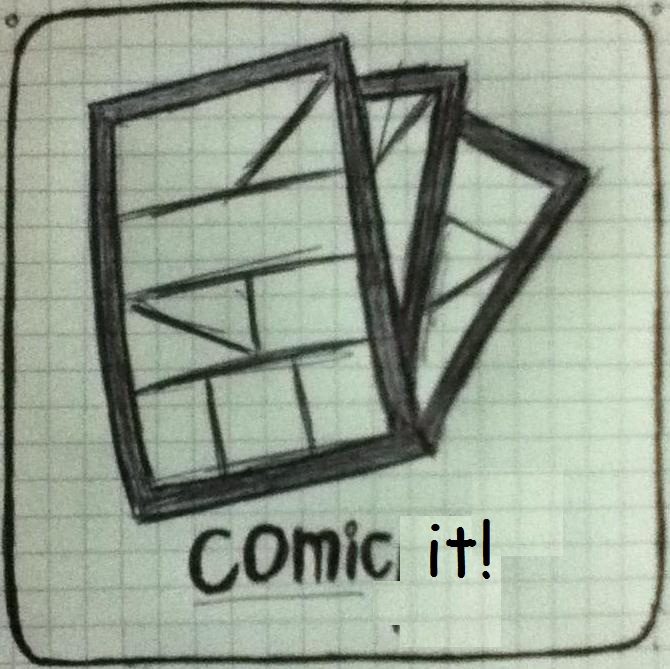
\includegraphics[width=0.45\textwidth]{comicit.jpg} %Midifico el width para cambiar el tamaño%
		\end{center}
	\end{frame}
	\begin{frame}
		\frametitle{
			\color{red}\textbf{\begin{center}{\huge{Funcionalidades}}\end{center}}
			\color{blue}\textbf{\begin{center}{\huge{¡Haz que tu imagen pase de ser buena a ser 								increíble!}}\end{center}}}
			\begin{center}
			\begin{itemize}
			\item\textbf{ EDICIÓN DE IMAGENES:}
			\newline
			Una opción que permite colocar efectos a la imagen que  desees,
			\newline
			 entre estos efectos tenemos Sepia, Blanco y Negro;  modificar el 
			\newline
			brillo, contraste, entre otras características de la imagen.
			\end{itemize}
		\end{center} 
	\end{frame}
	\begin{frame}
		\begin{center} 
				 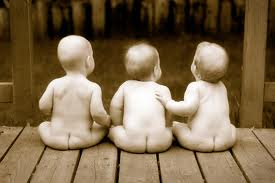
\includegraphics[width=0.45\textwidth]{images.jpg} %Midifico el width para cambiar el tamaño%
				 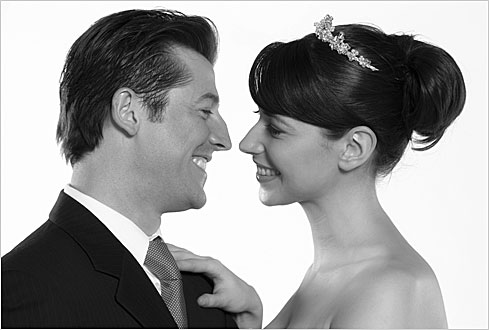
\includegraphics[width=0.45\textwidth]{4.jpg} %Midifico el width para cambiar el tamaño%
				 \newline				 
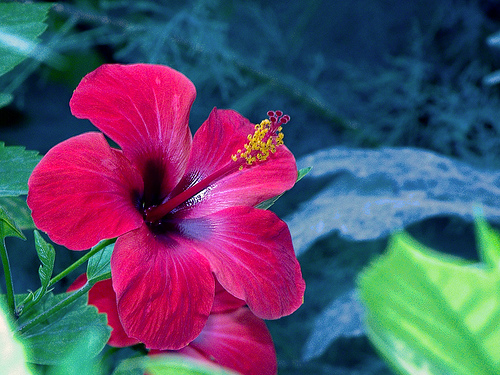
\includegraphics[width=0.45\textwidth]{5.jpg} %Midifico el width para cambiar el tamaño%
		\end{center}
	\end{frame}

	\begin{frame}
		\frametitle{
			\color{red}\textbf{\begin{center}{\huge{Funcionalidades}}\end{center}}
			\color{blue}\textbf{\begin{center}{\huge{Crea el diálogo de tus personajes}}\end{center}}}
			\begin{center}
			\begin{itemize}
			\item\textbf{LISTA DE BURBUJAS DE DIÁLOGO:}
			\newline
			Proporcionamos una lista con varios formatos de burbujas de
			\newline
			 diálogo, de las cuales el usuario puede escoger las que más  
			\newline
			se ajuste a su necesidad.
			\item\textbf{EDICIÓN DE BURBUJAS DE DIÁLOGO:}
			\newline
			El usuario podrá editar el texto dentro de la burbuja de diálogo 
			\newline
			que haya escogido, con la fuente, tamaño y color que desee.
			\end{itemize}
		\end{center} 
	\end{frame}	
	\begin{frame}
			\begin{center}
			\begin{itemize}
			\item\textbf{LISTA DE ICONOS:}
			\newline
			Proporcionamos una lista de iconos básicos y personalizados que
			\newline
			 permitirán al usuario crear imágenes más reales y divertidas.
			\newline
			\newline
			\item\textbf{EDICIÓN DE TEXTO O TEXTO PREDETERMINADO:}
			\newline
			Además de íconos, el usuario tendrá una lista de textos divertidos
			\newline
			para darle más creatividad a las escenas que esté creando. Si el u
			\newline
			 suario desea crear nuevos diseños tendrá la opción de hacer sus 
			\newline
			 propios dibujos y colocarlos en la imagen al igual que los iconos.
			\end{itemize}
		\end{center} 
	\end{frame}	
	\begin{frame}
	\begin{center}
		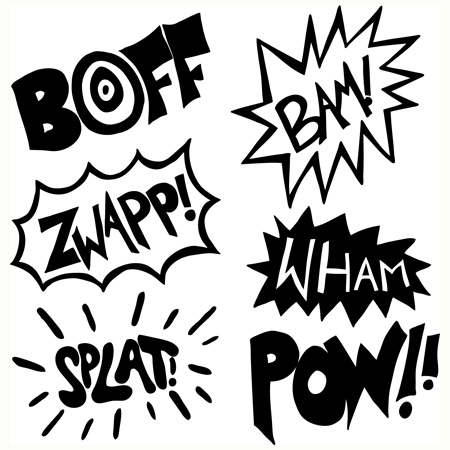
\includegraphics[width=0.45\textwidth]{6.jpg} %Midifico el width para cambiar el tamaño%
	\end{center}
	\end{frame}	
=======
=======
>>>>>>> f13d65079c56d991fba2a1e321ddf3aefe9887f4
=======
>>>>>>> f13d65079c56d991fba2a1e321ddf3aefe9887f4
		
		\color{blue}\textbf{\begin{center}{\Huge{¡Creando Historietas!}}\end{center}}
			
		
		
		\pause
		\begin{center} 
				 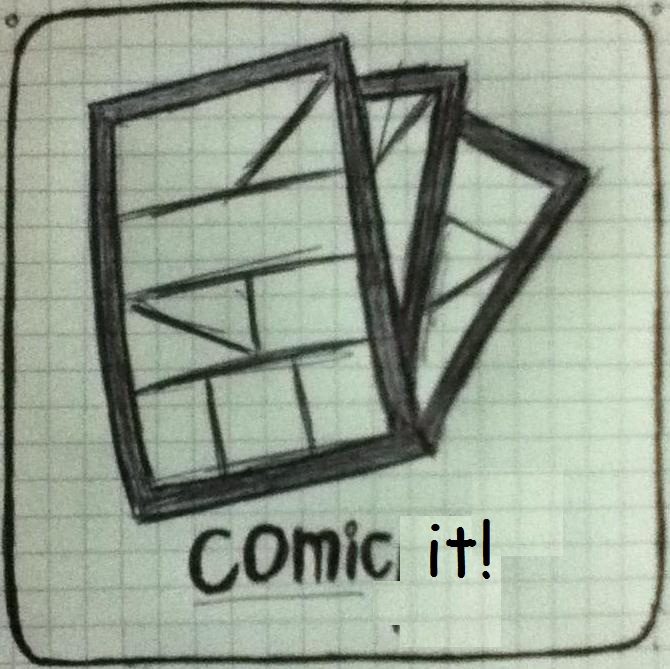
\includegraphics[width=0.5\textwidth]{comicit.jpg} %Midifico el width para cambiar el tamaño%
		\end{center}
	\end{frame}
	\begin{frame}	
	 	
		\color{blue}\textbf{\begin{center}{\Huge{Autores}}\end{center}}
		\color{black}
		\begin{center}\huge{ 
			\pause
			- Ana Arias\\
			\pause
			- Liliana Ramos\\
			\pause
			- Denny Schuldt
			
			\pause
		}
			\normalsize
			\vspace{9mm}
			 Lenguajes de Programación
			\\2012 - II Término

			
		\end{center}	
			
	\end{frame}
	\begin{frame}
		\textbf{Funcionalidades}
		\newline
		\begin{itemize}
			\item Funcionalidad 1
			\newline
			Hace x1 cosa con y1 parte de z1 dispositivo...
			\pause
			\item Funcionalidad 2
			\newline
			Hace x2 cosa con y2 parte de z2 dispositivo...
			\pause
			\item Funcionalidad 3
			\newline
			Hace x3 cosa con y3 parte de z3 dispositivo...
			\pause
			\newline
			\newline
			\newline
			\flushright
			...Wow!
		\end{itemize}
	\end{frame}	
	\begin{frame}
		\textbf{Como funciona?}
		\newline
		\newline
		%Colocar aqui el modo de funcionamiento esperado.%
		sdfvghaj  qfhnwjglj fhban yvawjhbs hteggdj ushf sdfvghaj  qfhnwjglj fhban yvawjhbs hteggdj ushf
		sdfvghaj  qfhnwjglj fhban yhbs hteggdj ushf sdfvghaj  qfhnwjglj fhban yvawjhbs hteggdj ushf
		sdfaj  qfhnwjglj fhban yvawjhbs hteggdj ushf.
		sdfvghaj  qfhnwjglj fhbahbs hteggdj ushf sdfvghaj  qfhnwjglj fhban yvawjhbs hteggdj ushf
		sdfvghaj  qfhnwjglj fhban yvahbs hteggdj ushf sdfvghaj  qfhnwjglj fhban yvawjhbs hteggdj ushf
		sdfvghaj  qfhnwjglj fhban yvawhbs hteggdj ushf sdfvghaj  qfhnwjglj fhban yvawjhbs hteggdj ushf
		hteggdj ushf sdfvghaj  qfhnwjglj fhban yvawjhbs hteggdj ush.
		%Hasta aquí la parte de funcionamiento.%
	\end{frame}
<<<<<<< HEAD
<<<<<<< HEAD
>>>>>>> f13d65079c56d991fba2a1e321ddf3aefe9887f4
=======
>>>>>>> f13d65079c56d991fba2a1e321ddf3aefe9887f4
=======
>>>>>>> f13d65079c56d991fba2a1e321ddf3aefe9887f4
	\begin{frame}
		\textbf{Ejemplos de plantillas:}
		\newline	
		\begin{center} 
			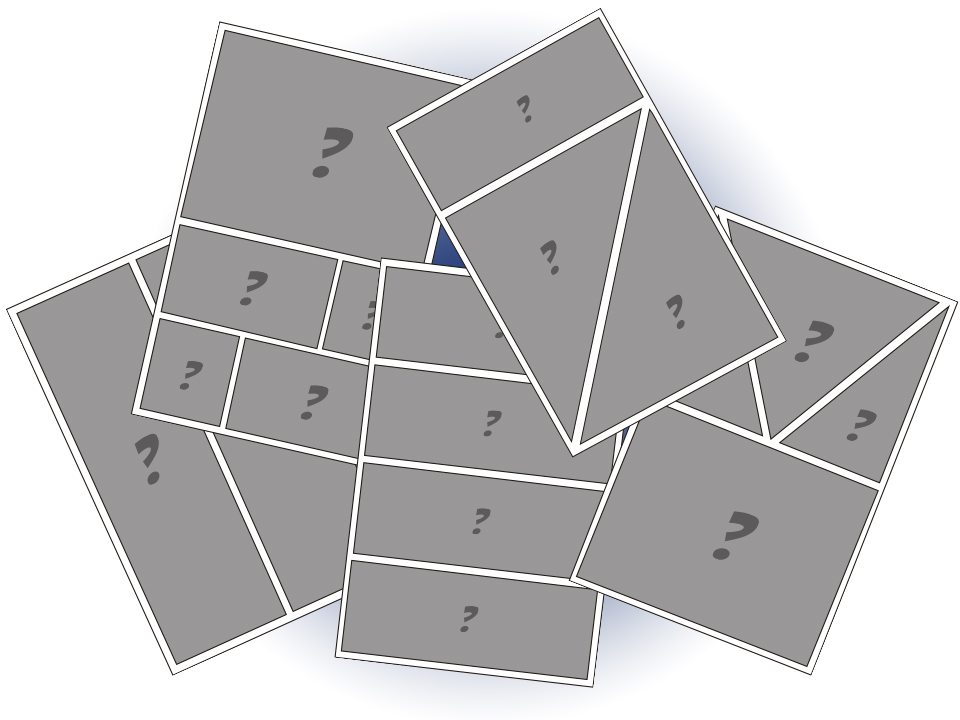
\includegraphics[width=0.8\textwidth]{plantillas.jpg}
		\end{center}
	\end{frame}
	\begin{frame}
		\transdissolve
		 
\includegraphics[width=1\textwidth]{failure.jpg} %Midifico el width para cambiar el tamaño%
	\end{frame}
\end{document}

